\documentclass[12pt, a4paper]{article}

% ── Margins ──────────────────────────────────────────────────────────────────
\usepackage[top=2.5cm, bottom=2.5cm, left=2.5cm, right=2.5cm]{geometry}

% ── Font & Language ──────────────────────────────────────────────────────────
\usepackage{polyglossia}
\setmainlanguage{greek}
\setotherlanguage{english}
\setmainfont{CMU Serif}
\setsansfont{CMU Sans Serif}
\setmonofont{CMU Typewriter Text}
\newfontfamily\greekfonttt{CMU Typewriter Text}
\newfontfamily\greekfontsf{CMU Sans Serif}
\newfontfamily\greekfont{CMU Serif}

% ── Line spacing ─────────────────────────────────────────────────────────────
\usepackage{setspace}
\setstretch{1.15}

% ── Math ─────────────────────────────────────────────────────────────────────
\usepackage{amsmath}
\usepackage{amssymb}

% ── Graphics & Figures ───────────────────────────────────────────────────────
\usepackage{graphicx}
\graphicspath{{./pictures/}}
\usepackage{caption}
\usepackage{subcaption}
\captionsetup{
    font=small,
    labelfont=bf,
    labelsep=period,
    justification=centering
}
\usepackage{float}

% ── Tables ───────────────────────────────────────────────────────────────────
\usepackage{booktabs}
\usepackage{array}

% ── Code listings ────────────────────────────────────────────────────────────
\usepackage{minted}
\setminted{
    fontsize=\small,
    frame=lines,
    framesep=6pt,
    linenos,
    breaklines
}

% ── Section styling ──────────────────────────────────────────────────────────
\usepackage{titlesec}
\titleformat{\section}{\large\bfseries}{\thesection.}{0.6em}{}[\titlerule]
\titleformat{\subsection}{\normalsize\bfseries}{\thesubsection}{0.6em}{}
\titleformat{\subsubsection}{\normalsize\itshape}{\thesubsubsection}{0.6em}{}
\titlespacing{\section}{0pt}{1.4em}{0.6em}
\titlespacing{\subsection}{0pt}{1em}{0.4em}
\titlespacing{\subsubsection}{0pt}{0.8em}{0.2em}

% ── Header / Footer ──────────────────────────────────────────────────────────
\usepackage{fancyhdr}
\pagestyle{fancy}
\fancyhf{}
\renewcommand{\headrulewidth}{0.4pt}
\fancyhead[L]{\small\textit{Όραση Υπολογιστών - 1η Εργαστηριακή Άσκηση}}
\fancyhead[R]{\small\textit{ΕΜΠ ΗΜΜΥ, 2025-2026}}
\fancyfoot[C]{\thepage}

% ── Misc ─────────────────────────────────────────────────────────────────────
\usepackage{xcolor}
\usepackage{ragged2e}
\usepackage{microtype}
\usepackage{hyperref}
\hypersetup{
    colorlinks=true,
    linkcolor=blue!70!black,
    urlcolor=blue!70!black,
    citecolor=green!50!black
}

% ── Layout ───────────────────────────────────────────────────────────────────
\setlength{\parindent}{0pt}
\setlength{\parskip}{0.5em}

% ─────────────────────────────────────────────────────────────────────────────
\begin{document}

% ── Title page ───────────────────────────────────────────────────────────────
\begin{titlepage}
    \begin{center}

        \begin{minipage}{0.3\textwidth}
            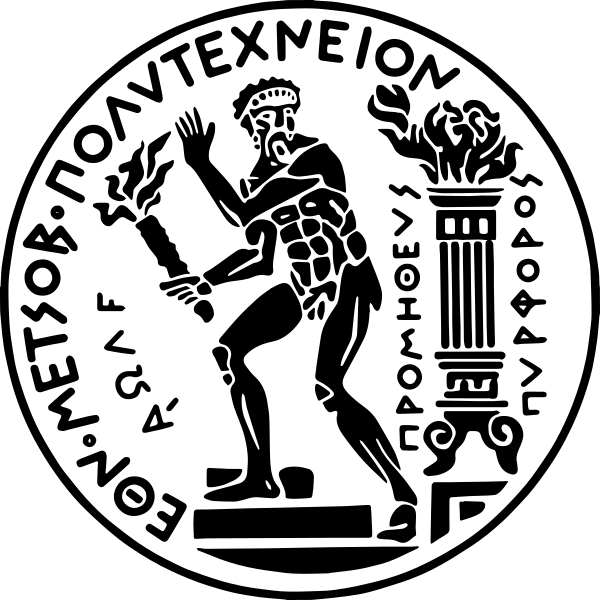
\includegraphics[width=\linewidth]{ntua_logo.png}
        \end{minipage}
        \hfill
        \begin{minipage}{0.65\textwidth}
            \centering
            {\LARGE \textbf{Εθνικό Μετσόβιο Πολυτεχνείο}}\\[0.3cm]
            {\large \textbf{Σχολή Ηλεκτρολόγων Μηχανικών \& Μηχανικών Υπολογιστών}}\\[0.2cm]
            \rule{\linewidth}{0.5pt}\\[0.3cm]
            {\large Εξάμηνο 8\textsuperscript{o}}\\[0.1cm]
            {\large \textbf{Όραση Υπολογιστών}}\\
        \end{minipage}

        \vspace{3cm}

        {\Huge \textbf{1η Εργαστηριακή Άσκηση}}\\[0.8cm]
        \rule{0.6\linewidth}{0.8pt}\\[0.8cm]
        {\LARGE \textbf{Εντοπισμός Σημείων Ενδιαφέροντος\\[0.3cm]
        και Εξαγωγή Χαρακτηριστικών σε Εικόνες}}\\[0.8cm]
        \rule{0.6\linewidth}{0.8pt}

        \vspace{4cm}

        {\large \textbf{Μέλη Ομάδας}}\\[0.6cm]
        \begin{tabular}{rl}
            \textbf{Καβαδάκης Σωτήρης}   & 03122035 \\[0.3cm]
            \textbf{Δαλαμπέκης Ιγνάτιος} & 03122017 \\
        \end{tabular}

        \vfill

        {\large Αθήνα, Μάρτιος 2026}

    \end{center}
\end{titlepage}
\clearpage

% ── Table of Contents ────────────────────────────────────────────────────────
\tableofcontents
\clearpage

% ─────────────────────────────────────────────────────────────────────────────
\section{Ανίχνευση Ακμών σε Γκρίζες Εικόνες}

\subsection{Δημιουργία Εικόνων Εισόδου}

\subsubsection{Φόρτωση Αρχικής Εικόνας}

Φορτώθηκε η αρχική γκρίζα εικόνα $I_0 = $ \texttt{edgetest\_26.png} με χρήση της συνάρτησης
\texttt{cv2.imread} με τη σημαία \texttt{IMREAD\_GRAYSCALE}, ώστε να διαβαστεί απευθείας
ως εικόνα grayscale. Στη συνέχεια μετατράπηκε σε τύπο \texttt{float64} για ακρίβεια
στους υπολογισμούς που ακολουθούν και αποφυγή overflow.

\subsubsection{Προσθήκη Θορύβου}

Για την αξιολόγηση της ανθεκτικότητας των αλγορίθμων ανίχνευσης ακμών, δημιουργήθηκαν
δύο θορυβώδεις εκδόσεις της $I_0$ με την πρόσθεση λευκού Gaussian θορύβου:
\begin{equation}
    I(x, y) = I_0(x, y) + n(x, y), \quad n(x,y) \sim \mathcal{N}(0,\, \sigma_n^2)
\end{equation}


Το PSNR (Peak Signal-to-Noise Ratio) ορίζεται ως:
\begin{equation}
    \text{PSNR} = 20\log_{10}\!\left(\frac{I_{\max} - I_{\min}}{\sigma_n}\right) \quad [\text{dB}]
\end{equation}
όπου $I_{\max}$ και $I_{\min}$ είναι η μέγιστη και ελάχιστη τιμή της $I_0$.
Αντιστρέφοντας τη σχέση αυτή προκύπτει:
\begin{equation}
    \sigma_n = \frac{I_{\max} - I_{\min}}{10^{\,\text{PSNR}/20}}
\end{equation}
Χρησιμοποιήθηκαν δύο τιμές: $\text{PSNR} = 20\,\text{dB}$ και $\text{PSNR} = 10\,\text{dB}$,
παράγοντας τις εικόνες $I_{20}$ και $I_{10}$ αντίστοιχα.

Καθώς το PSNR μετρά λογαριθμικά τον λόγο σήματος-προς-θόρυβο, μείωση κατά
$10\,\text{dB}$ αντιστοιχεί σε τριπλασιασμό ($\times 10^{10/20} \approx 3.16$) της τυπικής
απόκλισης $\sigma_n$. Έτσι η $I_{10}$ έχει σημαντικά πιο έντονο θόρυβο από την $I_{20}$,
κάτι που είναι εμφανές στο Σχήμα~\ref{fig:noisy}: στην $I_{10}$ τα ομοιόμορφα τμήματα
της εικόνας εμφανίζουν έντονη κοκκώδη υφή, ενώ στην $I_{20}$ ο θόρυβος είναι ήπιος.
Η επιλογή Gaussian θορύβου είναι θεωρητικά ενδιαφέρουσα διότι αποτελεί το χειρότερο
δυνατό θόρυβο για δεδομένη ισχύ (μέγιστη εντροπία), οπότε αποτελεί αυστηρό κριτήριο
ανθεκτικότητας για τον αλγόριθμο ανίχνευσης ακμών.

\begin{figure}[H]
    \centering
    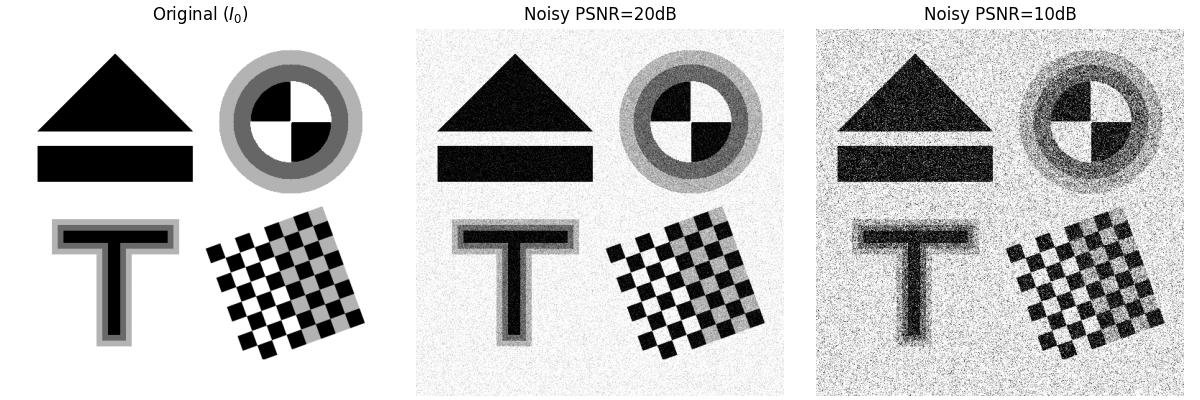
\includegraphics[width=\linewidth]{noisy_images.jpg}
    \caption{Αρχική εικόνα $I_0$ (αριστερά), θορυβώδης εικόνα $I_{20}$ με PSNR = 20 dB
             (κέντρο) και $I_{10}$ με PSNR = 10 dB (δεξιά). Η αύξηση του θορύβου είναι
             εμφανής στη μεταβολή της ομοιόμορφης υφής.}
    \label{fig:noisy}
\end{figure}

\subsection{Υλοποίηση Αλγορίθμων Ανίχνευσης Ακμών}

Η μέθοδος που υλοποιείται βασίζεται στον αλγόριθμο Marr-Hildreth \cite{marr1980},
ο οποίος προτάθηκε το 1980 ως βιολογικά εμπνευσμένο μοντέλο ανίχνευσης ακμών.
Η κεντρική ιδέα είναι ότι η ανθρώπινη όραση επεξεργάζεται εικόνες σε πολλαπλές
χωρικές κλίμακες μέσω κυψελιδωτών πεδίων που προσεγγίζονται από το LoG, και
εντοπίζει ακμές στα zero-crossings της εξόδου. Ο αλγόριθμος αποτελείται από τα
βήματα που περιγράφονται στις ακόλουθες υποενότητες.

\subsubsection{Πυρήνες Gaussian και LoG}

Η ανίχνευση ακμών μέσω zero-crossings της Laplacian απαιτεί δύο φίλτρα: έναν πυρήνα
Gaussian $G_\sigma$ για εξομάλυνση της εικόνας, και έναν πυρήνα Laplacian-of-Gaussian
(LoG) $h = \nabla^2 G_\sigma$ για την εκτίμηση της δεύτερης παραγώγου.

Ο πυρήνας $G_\sigma$ κατασκευάστηκε εκμεταλλευόμενος την ιδιότητα διαχωρισιμότητας
της 2D Gaussian: επειδή $G_\sigma(x,y) = G_\sigma(x)\cdot G_\sigma(y)$, ο 2D πυρήνας
προκύπτει ως εξωτερικό γινόμενο δύο 1D πυρήνων που επιστρέφει η \texttt{cv2.getGaussianKernel}.
Αυτό είναι υπολογιστικά αποδοτικότερο από την άμεση κατασκευή του 2D πυρήνα.

Ο πυρήνας LoG υπολογίστηκε απευθείας από τον αναλυτικό τύπο που προκύπτει
εφαρμόζοντας τον τελεστή Laplace στη 2D Gaussian:
\begin{equation}
    h(x,y) = \nabla^2 G_\sigma(x,y)
           = \frac{r^2 - 2\sigma^2}{2\pi\sigma^6}\,
             \exp\!\left(-\frac{r^2}{2\sigma^2}\right), \quad r^2 = x^2 + y^2
\end{equation}
Και στις δύο περιπτώσεις, το μέγεθος του πυρήνα ορίστηκε ως $n = 2\lceil 3\sigma \rceil + 1$,
ώστε να καλύπτεται εύρος $\pm 3\sigma$ γύρω από το κέντρο — περιοχή που εμπεριέχει
$99.7\%$ της ενέργειας της Gaussian. Χρήση μικρότερου πυρήνα θα εισήγαγε
σφάλμα αποκοπής (truncation error), ενώ μεγαλύτερος πυρήνας θα αύξανε
αχρείαστα τον υπολογιστικό κόστος.

Επιπλέον, ο πυρήνας LoG κεντράρεται ως προς το μηδέν με την αφαίρεση της μέσης
τιμής του (\texttt{kernel -= kernel.mean()}). Αυτό είναι θεωρητικά αναγκαίο: ο
ιδανικός πυρήνας LoG ικανοποιεί $\int\!\int h(x,y)\,dx\,dy = 0$, οπότε η
απόκρισή του σε σταθερές περιοχές είναι μηδέν. Στη διακριτή προσέγγιση με
περικομμένο πυρήνα αυτή η ιδιότητα δεν ικανοποιείται ακριβώς, και η διόρθωση
αποτρέπει την εισαγωγή DC offset στην εκτίμηση της Laplacian.

\subsubsection{Προσέγγιση Laplacian}

Για την εκτίμηση της Laplacian της εξομαλυμένης εικόνας $I_\sigma = G_\sigma * I$
υλοποιήθηκαν δύο εναλλακτικές προσεγγίσεις. Η εξομάλυνση με Gaussian είναι
θεμελιώδης στη μέθοδο: η Laplacian είναι τελεστής δεύτερης παραγώγου και ως εκ
τούτου εξαιρετικά ευαίσθητος στον θόρυβο, καθώς η παραγώγιση ενισχύει τις υψηλές
συχνότητες. Η προηγούμενη εξομάλυνση με $G_\sigma$ καταστέλλει τον θόρυβο
ελέγχοντας αυτές τις συχνότητες, ενώ η κλίμακα $\sigma$ καθορίζει τον βαθμό
εξομάλυνσης και άρα την ανθεκτικότητα έναντι θορύβου σε βάρος της χωρικής
ακρίβειας εντοπισμού των ακμών.

Η πρώτη, \textbf{γραμμική} ($L_1$), εκμεταλλεύεται την ιδιότητα της συνέλιξης ότι
ο τελεστής Laplace επιτρέπει εναλλαγή με τη συνέλιξη:
\begin{equation}
    L_1 = \nabla^2(G_\sigma * I) = (\nabla^2 G_\sigma) * I = h * I
\end{equation}
Έτσι αρκεί μία μόνο συνέλιξη της εικόνας εισόδου $I$ με τον πυρήνα LoG $h$,
αντί για ξεχωριστή εξομάλυνση και εφαρμογή Laplacian.

Η δεύτερη, \textbf{μη-γραμμική} ($L_2$), βασίζεται σε μορφολογικούς τελεστές
\cite{maragos2005} εφαρμοζόμενους στην ήδη εξομαλυμένη εικόνα $I_\sigma$:
\begin{equation}
    L_2 = (I_\sigma \oplus B) + (I_\sigma \ominus B) - 2I_\sigma
\end{equation}
όπου $B$ είναι στοιχείο δόμησης $3\times3$. Εδώ η εξομάλυνση πρέπει να εφαρμοστεί
\emph{ρητά} πριν τους μορφολογικούς τελεστές, αφού — σε αντίθεση με την $L_1$ —
δεν υπάρχει δυνατότητα ενοποίησης των δύο βημάτων σε έναν ενιαίο πυρήνα λόγω
της μη-γραμμικότητας των τελεστών max/min \cite{maragos2005}. Η φυσική ερμηνεία
της έκφρασης είναι ανάλογη με τον κλασικό τύπο διακριτής δεύτερης παραγώγου
$f(x+h) + f(x-h) - 2f(x) \approx h^2 f''(x)$, με τη dilation και erosion να
παίζουν τον ρόλο των τοπικών μεγίστων και ελαχίστων αντίστοιχα.

\subsubsection{Εύρεση Zero-crossings}

Τα σημεία μηδενισμού (zero-crossings) της Laplacian $L$ αντιστοιχούν στις ακμές
της εξομαλυμένης εικόνας. Η βασική ιδέα είναι ότι σε κάθε ακμή η εικόνα
παρουσιάζει απότομη μεταβολή έντασης, η πρώτη παράγωγός της έχει τοπικό
μέγιστο, και συνεπώς η δεύτερη παράγωγος (Laplacian) αλλάζει πρόσημο —
δηλαδή διέρχεται από το μηδέν. Εντοπίζοντας αυτές τις διαβάσεις από το μηδέν
βρίσκουμε τις ακμές με υποπixel ακρίβεια, σε αντίθεση με μεθόδους που ψάχνουν
τοπικά μέγιστα της κλίσης.

Ο εντοπισμός υλοποιείται σε δύο βήματα. Πρώτα κατασκευάζεται η δυαδική
εικόνα προσήμου $X = (L \geq 0)$, όπου τα pixels με $L \geq 0$ παίρνουν τιμή 1
και τα υπόλοιπα τιμή 0. Τα zero-crossings βρίσκονται ακριβώς στα όρια μεταξύ
περιοχών τιμής 0 και 1 στην $X$, δηλαδή στο μορφολογικό όριο $\partial X$ του
συνόλου $X$. Σύμφωνα με τη θεωρία μαθηματικής μορφολογίας \cite{maragos2005},
το όριο ενός δυαδικού συνόλου προσεγγίζεται ως:
\begin{equation}
    Y = (X \oplus B) - (X \ominus B) \approx \partial X
\end{equation}
Τα pixels όπου $Y = 1$ αποτελούν τα zero-crossings της $L$. Η συμμετρία της
έκφρασης — dilation που διαστέλλει το σύνολο $X$ και erosion που το συρρικνώνει
— εξασφαλίζει ότι το εξαγόμενο όριο είναι συμμετρικό ως προς το $X$ και το
συμπλήρωμά του $X^c$ \cite{maragos2005}, αποφεύγοντας συστηματική μετατόπιση
των ακμών προς τη μία ή την άλλη πλευρά.

\subsubsection{Απόρριψη σε Ομαλές Περιοχές}

Τα zero-crossings της Laplacian εμφανίζονται σε κάθε σημείο αλλαγής προσήμου,
ακόμη και σε ομαλές περιοχές όπου η Laplacian ταλαντώνεται γύρω από το μηδέν
λόγω θορύβου. Αυτά τα ψευδή zero-crossings δεν αντιστοιχούν σε πραγματικές
ακμές και πρέπει να απορριφθούν. Ο μηχανισμός που χρησιμοποιείται βασίζεται
στην κλίση (gradient magnitude) της εξομαλυμένης εικόνας $I_\sigma$: μια
πραγματική ακμή συνοδεύεται αναγκαστικά από μεγάλη κλίση, ενώ σε ομαλές
περιοχές η κλίση είναι μικρή. Συγκεκριμένα, η τελική δυαδική εικόνα ακμών $D$
προκύπτει ως:
\begin{equation}
    D[i,j] = 1 \iff Y[i,j] = 1 \;\text{και}\;
    \|\nabla I_\sigma[i,j]\| > \theta_{\text{edge}} \cdot \max_{x,y} \|\nabla I_\sigma\|
\end{equation}
Η κλίση $\|\nabla I_\sigma\| = \sqrt{(\partial I_\sigma / \partial x)^2 +
(\partial I_\sigma / \partial y)^2}$ υπολογίζεται στην εξομαλυμένη (και όχι στην
αρχική) εικόνα, γιατί η εξομάλυνση έχει ήδη καταστείλει τον θόρυβο, οπότε η
κλίση αντικατοπτρίζει πραγματικές μεταβάσεις έντασης.

Η επιλογή του $\|\nabla I_\sigma\|$ ως κριτηρίου απόρριψης — αντί της απόλυτης
τιμής της Laplacian $|L|$ — είναι σκόπιμη: το $|L|$ είναι μηδέν ακριβώς στα
zero-crossings (εξ ορισμού), οπότε δεν παρέχει κανένα διαχωριστικό κριτήριο
εκεί. Αντίθετα, η κλίση $\|\nabla I_\sigma\|$ είναι τοπικά μέγιστη στα σημεία
που αντιστοιχούν σε πραγματικές ακμές και μικρή στα ψευδή zero-crossings που
οφείλονται σε θόρυβο, επιτρέποντας τη διάκρισή τους.

Η παράμετρος $\theta_{\text{edge}} \in [0,1]$ ελέγχει την αυστηρότητα: υψηλότερη
τιμή κρατά μόνο τις ισχυρότερες ακμές μειώνοντας τον θόρυβο αλλά χάνοντας
ασθενείς ακμές, ενώ χαμηλή τιμή ανιχνεύει περισσότερες ακμές αλλά εισάγει
ψευδοανιχνεύσεις. Η βέλτιστη τιμή εξαρτάται από το επίπεδο θορύβου της
εικόνας εισόδου.

\subsection{Αξιολόγηση Αποτελεσμάτων}

\subsubsection{Υπολογισμός Αληθινών Ακμών}

Για να αξιολογηθεί ποσοτικά ο αλγόριθμος ανίχνευσης ακμών, χρειάζεται μια
δυαδική εικόνα αληθινών ακμών $T$ (ground truth). Αφού διαθέτουμε την αρχική
καθαρή εικόνα $I_0$ χωρίς θόρυβο, οι αληθινές ακμές μπορούν να εκτιμηθούν
μέσω της μορφολογικής κλίσης (morphological gradient) \cite{maragos2005}:
\begin{equation}
    M = (I_0 \oplus B) - (I_0 \ominus B)
\end{equation}
Η ποσότητα $M$ μετρά σε κάθε pixel τη μέγιστη μεταβολή έντασης εντός
γειτονιάς $3 \times 3$: σε ομαλές περιοχές η dilation και η erosion δίνουν
παρόμοιες τιμές ($M \approx 0$), ενώ στις ακμές η διαφορά τους είναι μεγάλη.
Η τελική δυαδική εικόνα αληθινών ακμών προκύπτει με κατωφλιοποίηση:
$T = (M > \theta_{\text{real}} \cdot \max M)$, με
$\theta_{\text{real}} = 0.1$.

\subsubsection{Ποσοτική Αξιολόγηση}

Η σύγκριση μεταξύ των ανιχνευθεισών ακμών $D$ και των αληθινών $T$ γίνεται
μέσω του κριτηρίου:
\begin{equation}
    C = \frac{Pr(D|T) + Pr(T|D)}{2} = \frac{\text{Precision} + \text{Recall}}{2}
\end{equation}
όπου $\text{Precision} = |D \cap T| / |D|$ είναι το ποσοστό ανιχνευθεισών
ακμών που είναι πραγματικά ακμές, και $\text{Recall} = |D \cap T| / |T|$
το ποσοστό αληθινών ακμών που εντοπίστηκαν. Το κριτήριο $C$ ισορροπεί
μεταξύ αυτών των δύο ποσοτήτων: ένας αλγόριθμος που ανιχνεύει πάρα πολλές
ακμές μπορεί να πετύχει υψηλό Recall αλλά θα έχει χαμηλό Precision (πολλές
ψευδοανιχνεύσεις), ενώ ένας υπερβολικά συντηρητικός αλγόριθμος θα έχει υψηλό
Precision αλλά χαμηλό Recall (χάνει ακμές). Η μέγιστη τιμή $C = 1$
αντιστοιχεί σε τέλεια ανίχνευση.

\subsubsection{Πειραματισμός Παραμέτρων}

Για κάθε επίπεδο θορύβου πειραματιστήκαμε με τις παραμέτρους $\sigma$ και
$\theta_{\text{edge}}$ ώστε να μεγιστοποιηθεί η μετρική $C$. Ως ενδεικτικές
τιμές αφετηρίας χρησιμοποιήθηκαν: $\sigma = 1.5$, $\theta_{\text{edge}} = 0.2$
για PSNR $= 20\,\text{dB}$ και $\sigma = 3.0$, $\theta_{\text{edge}} = 0.2$
για PSNR $= 10\,\text{dB}$, σύμφωνα με τις προτεινόμενες τιμές της εκφώνησης.
Τα αποτελέσματα φαίνονται στα Σχήματα~\ref{fig:edges_psnr20}
και~\ref{fig:edges_psnr10}.

\begin{figure}[H]
    \centering
    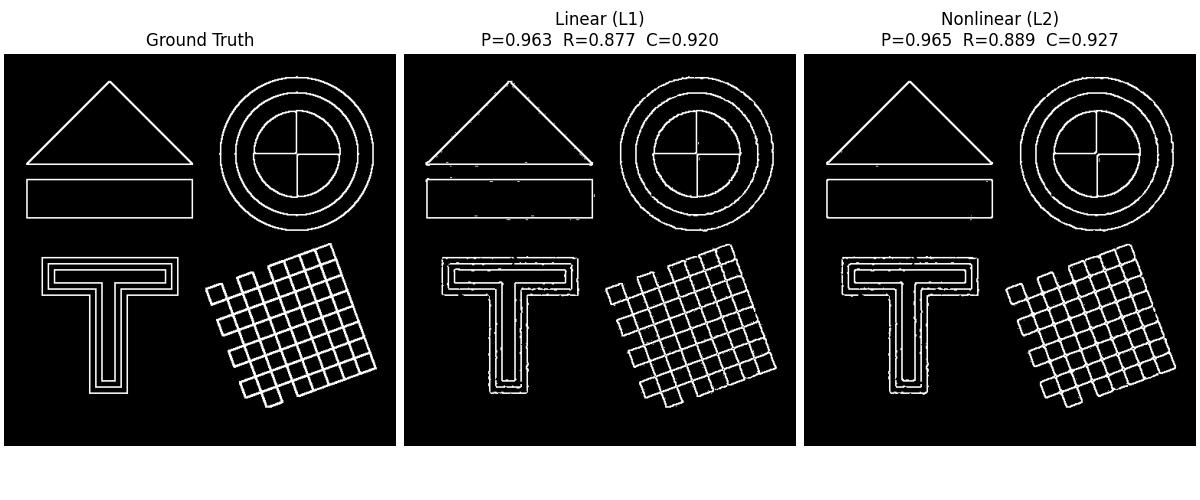
\includegraphics[width=\linewidth]{edges_PSNR20dB_sigma1.5_theta0.2.jpg}
    \caption{Αποτελέσματα ανίχνευσης ακμών για PSNR $= 20\,\text{dB}$,
             $\sigma = 1.5$, $\theta_{\text{edge}} = 0.2$. Αριστερά: αληθινές
             ακμές $T$, κέντρο: γραμμική μέθοδος ($L_1$), δεξιά: μη-γραμμική
             μέθοδος ($L_2$).}
    \label{fig:edges_psnr20}
\end{figure}

\begin{figure}[H]
    \centering
    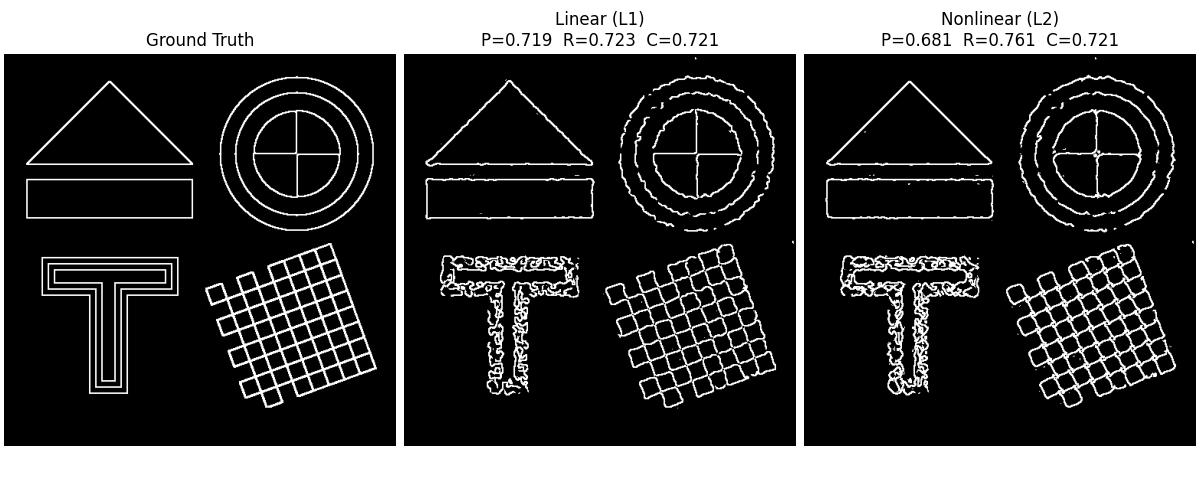
\includegraphics[width=\linewidth]{edges_PSNR10dB_sigma3.0_theta0.2.jpg}
    \caption{Αποτελέσματα ανίχνευσης ακμών για PSNR $= 10\,\text{dB}$,
             $\sigma = 3.0$, $\theta_{\text{edge}} = 0.2$. Η αύξηση του $\sigma$
             αντισταθμίζει τον ισχυρότερο θόρυβο, αλλά εισάγει μεγαλύτερη
             χωρική αβεβαιότητα στον εντοπισμό.}
    \label{fig:edges_psnr10}
\end{figure}

Η αύξηση του $\sigma$ στην περίπτωση PSNR $= 10\,\text{dB}$ είναι αναμενόμενη:
ο ισχυρότερος θόρυβος απαιτεί πιο επιθετική εξομάλυνση, που όμως πλαταίνει
τους πυρήνες φίλτρων και αμβλύνει τις ακμές. Αυτό αποτυπώνεται στα
αποτελέσματα, όπου οι ακμές στο PSNR $= 10\,\text{dB}$ είναι λιγότερο
ευκρινείς σε σύγκριση με αυτές στα $20\,\text{dB}$. Η γραμμική μέθοδος ($L_1$)
τείνει να δίνει πιο λεπτές ακμές, ενώ η μη-γραμμική ($L_2$) παράγει πιο
παχιές ακμές λόγω της φύσης των μορφολογικών τελεστών, που λαμβάνουν υπόψη
μόνο τις ακραίες τιμές (max/min) στη γειτονιά. Επιπλέον, κατασκευάστηκαν
καμπύλες Precision-Recall σαρώνοντας την $\theta_{\text{edge}}$
(Σχήμα~\ref{fig:pr_curves}), και παρουσιάζεται η μεταβολή της μετρικής $C$ ως
συνάρτηση του $\sigma$ (Σχήμα~\ref{fig:sigma_sweep}).

\begin{figure}[H]
    \centering
    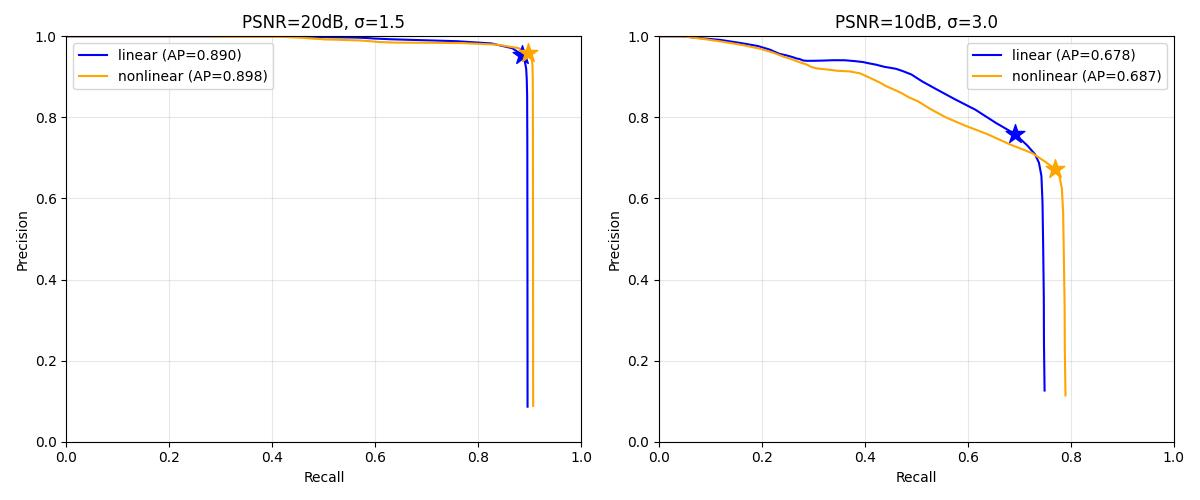
\includegraphics[width=\linewidth]{precision_recall_curves.jpg}
    \caption{Καμπύλες Precision-Recall για σάρωση του $\theta_{\text{edge}}$.
             Ο αστερίσκος σημειώνει το σημείο μέγιστου $C$.}
    \label{fig:pr_curves}
\end{figure}

\begin{figure}[H]
    \centering
    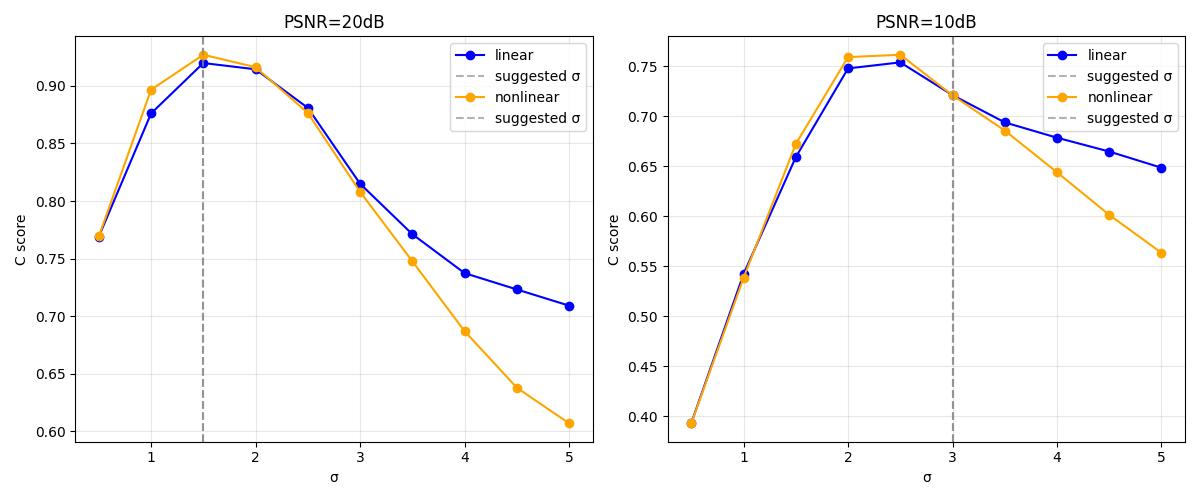
\includegraphics[width=\linewidth]{sigma_sweep.jpg}
    \caption{Μεταβολή της μετρικής $C$ συναρτήσει του $\sigma$ για
             $\theta_{\text{edge}} = 0.2$. Η κατακόρυφη γραμμή δείχνει
             την προτεινόμενη τιμή $\sigma$.}
    \label{fig:sigma_sweep}
\end{figure}

\subsection{Εφαρμογή σε Πραγματικές Εικόνες}

\subsubsection{Εφαρμογή στην \texttt{ermoupoli.jpg}}

Οι αλγόριθμοι ανίχνευσης ακμών εφαρμόστηκαν στην πραγματική εικόνα
\texttt{ermoupoli.jpg} χωρίς πρόσθεση τεχνητού θορύβου. Σε αντίθεση με τη
συνθετική εικόνα που περιέχει καθαρά γεωμετρικά σχήματα με ευδιάκριτες
μεταβάσεις, η πραγματική εικόνα παρουσιάζει ομαλές μεταβολές φωτεινότητας,
πολύπλοκες υφές και φυσικό θόρυβο, καθιστώντας την ανίχνευση ακμών
σημαντικά πιο απαιτητική. Η αξιολόγηση εδώ είναι αποκλειστικά ποιοτική
(οπτική), αφού δεν υπάρχει ground truth.

\subsubsection{Αξιολόγηση Αποτελεσμάτων}

Δοκιμάστηκαν τέσσερις συνδυασμοί παραμέτρων που καλύπτουν συστηματικά τον
χώρο παραμέτρων, ώστε να αναδειχθεί η επίδραση κάθε παραμέτρου ξεχωριστά.
Η εικόνα \texttt{ermoupoli.jpg} παρουσιάζει αρχιτεκτονική δομή (κτίριο,
παράθυρα, κολώνες) αλλά και δύσκολες περιοχές όπως βλάστηση και ουρανός,
προσφέροντας ένα αντιπροσωπευτικό πεδίο δοκιμής.

\begin{figure}[H]
    \centering
    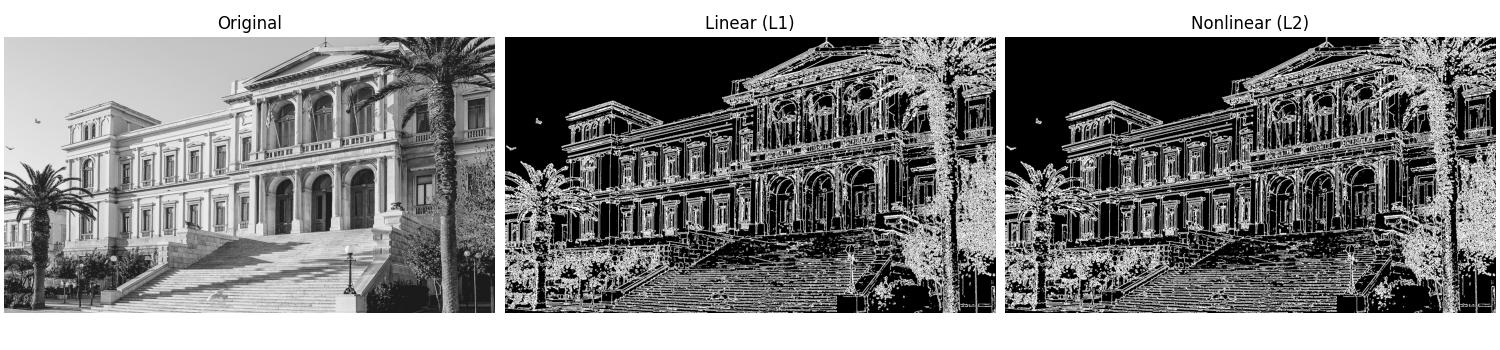
\includegraphics[width=\linewidth]{real_edges_sigma1.5_theta0.1.jpg}
    \caption{$\sigma=1.5$, $\theta_{\text{edge}}=0.1$. Το χαμηλό $\sigma$
             διατηρεί λεπτομέρεια και χωρική ακρίβεια, αλλά το χαμηλό
             κατώφλι αφήνει να περάσουν πολλές ψευδοανιχνεύσεις: η βλάστηση
             και η υφή της πρόσοψης δημιουργούν πυκνό θορυβώδη χάρτη
             zero-crossings που δυσχεραίνει την ανάγνωση των δομικών ακμών.}
    \label{fig:real_low_low}
\end{figure}

\begin{figure}[H]
    \centering
    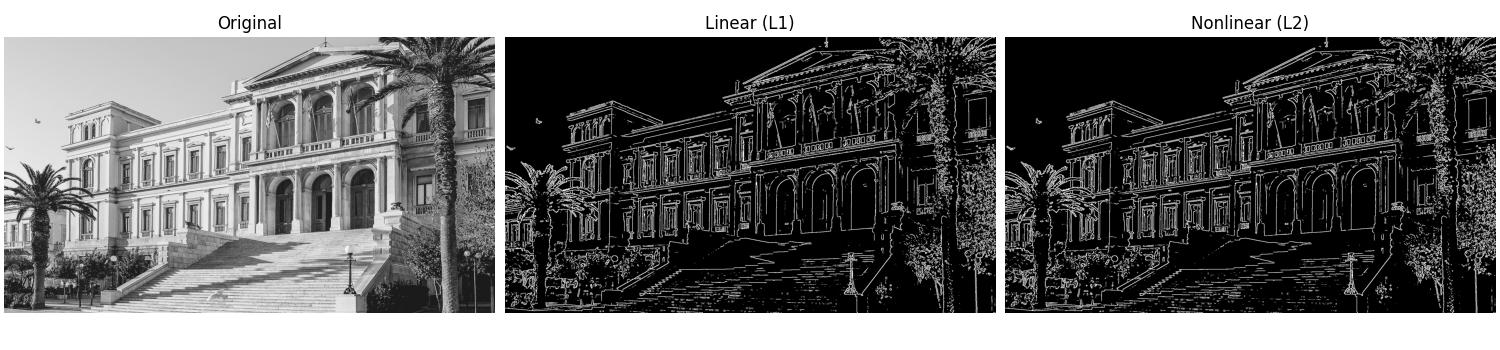
\includegraphics[width=\linewidth]{real_edges_sigma1.5_theta0.3.jpg}
    \caption{$\sigma=1.5$, $\theta_{\text{edge}}=0.3$ --- \textbf{καλύτερος
             συνδυασμός}. Η αύξηση του κατωφλίου εξαλείφει τις
             ψευδοανιχνεύσεις από υφές και θόρυβο, ενώ ο μικρός $\sigma$
             διατηρεί την ακρίβεια εντοπισμού: τα περιγράμματα του κτιρίου,
             τα παράθυρα και οι κολώνες αποδίδονται με καθαρές, λεπτές ακμές.}
    \label{fig:real_low_high}
\end{figure}

\begin{figure}[H]
    \centering
    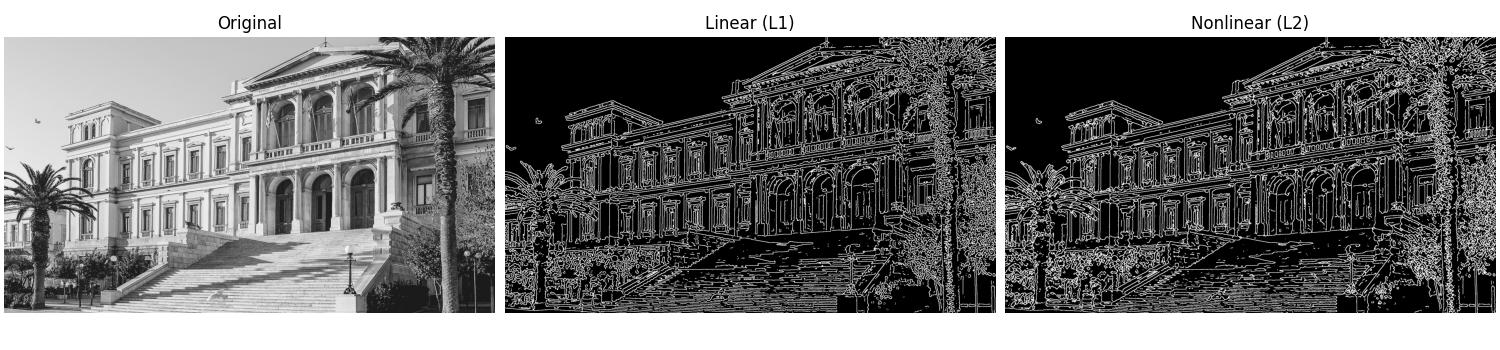
\includegraphics[width=\linewidth]{real_edges_sigma3.0_theta0.1.jpg}
    \caption{$\sigma=3.0$, $\theta_{\text{edge}}=0.1$. Η αυξημένη εξομάλυνση
             καταστέλλει αποτελεσματικά τον θόρυβο στη βλάστηση, αλλά
             πλαταίνει τις ακμές και συγχωνεύει γειτονικές δομές: τα μικρά
             παράθυρα χάνουν την ατομική τους ταυτότητα και τα λεπτά
             αρχιτεκτονικά στοιχεία γίνονται δυσδιάκριτα.}
    \label{fig:real_high_low}
\end{figure}

\begin{figure}[H]
    \centering
    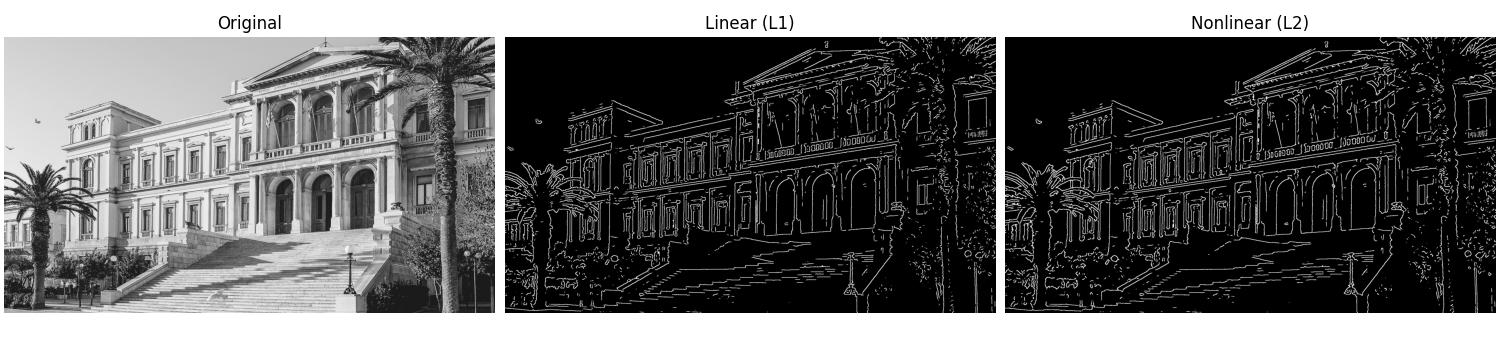
\includegraphics[width=\linewidth]{real_edges_sigma3.0_theta0.3.jpg}
    \caption{$\sigma=3.0$, $\theta_{\text{edge}}=0.3$. Ο πιο συντηρητικός
             συνδυασμός: απομένουν μόνο οι κυρίαρχες ακμές υψηλής κλίσης
             (κύριο περίγραμμα κτιρίου, ορίζοντας). Ο χάρτης είναι
             εξαιρετικά καθαρός αλλά αδυνατεί να αποδώσει οποιαδήποτε
             δομική λεπτομέρεια της εικόνας.}
    \label{fig:real_high_high}
\end{figure}

Ο καλύτερος συνδυασμός είναι $\sigma = 1.5$, $\theta_{\text{edge}} = 0.3$
(Σχήμα~\ref{fig:real_low_high}). Η επιλογή αυτή αξιοποιεί τον μικρό $\sigma$
για να διατηρήσει τη χωρική ακρίβεια — κρίσιμη για αρχιτεκτονικές δομές —
ενώ το υψηλότερο κατώφλι δρα ως εκλεκτικό φίλτρο που κρατά μόνο τα
zero-crossings με μεγάλη κλίση, δηλαδή αυτά που αντιστοιχούν σε πραγματικές
οπτικές ακμές. Αυτή η λογική είναι σύμφωνη με την πρόβλεψη του Marr-Hildreth
\cite{marr1980}: σε φυσικές εικόνες, τα όρια αντικειμένων συνοδεύονται από
σημαντικά μεγαλύτερη κλίση από ό,τι οι υφές ή ο θόρυβος.

Η σύγκριση $L_1$ και $L_2$ στην πραγματική εικόνα επιβεβαιώνει τα ευρήματα
της συνθετικής: η $L_1$ παράγει λεπτότερες, πιο συνεχείς ακμές, ενώ η $L_2$
δίνει παχύτερες και πιο αποσπασματικές. Για αρχιτεκτονικές εικόνες, όπου οι
ακμές είναι κυρίως μακριές και συνεχείς, η $L_1$ φαίνεται ποιοτικά ανώτερη.
Η $L_2$ μπορεί να προτιμηθεί όταν η ακρίβεια εντοπισμού σε επίπεδο pixel
είναι σημαντικότερη από τη συνέχεια.

% ─────────────────────────────────────────────────────────────────────────────
\clearpage
\begin{thebibliography}{9}

\bibitem{maragos2005}
Π. Μαραγκός,
\textit{Όραση Υπολογιστών: Κεφ.\ 7 - Τελεστές Δυαδικών Εικόνων \& Σχημάτων},
ΕΜΠ, 2005.

\bibitem{marr1980}
D. Marr and E. Hildreth,
Theory of edge detection,
\textit{Proceedings of the Royal Society of London B}, vol.\ 207, pp.\ 187--217, 1980.

\end{thebibliography}

\end{document}
